\newpage	
\section{Model Building and Solution}

\subsection{Model Establishment and Solution of Question One}
\subsubsection{Model Establishment}
Q1的目标是在题面未直接给出投票数/投票比例的条件下，为每个赛季-周-选手构造可用于后续机制对比的“观众偏好强度”后验分布。我们将\textbf{周淘汰结果}视为对观众偏好的一条弱监督约束，将\textbf{评委信号}作为技术线参考，并在每个\texttt{season$\times$week}上独立地推断一组粉丝份额（simplex）并量化不确定性。

\subsubsection{Inference mechanics (aligned to implementation)}
在实现上，我们对每个\texttt{season$\times$week}独立进行一次重要性抽样：

\paragraph{Step 1: prior draw (fan simplex)}
对当周在场选手集合（大小为$n$），从对称Dirichlet先验抽样得到$M$组候选观众份额向量：
\begin{equation}
\mathbf{p}^{(m)} \sim \mathrm{Dirichlet}(\mathbf{1}),\quad m=1,\dots,M.
\end{equation}

\paragraph{Step 2: combine judge and fan signals}
Percent机制下，我们将评委百分比$J_i$与候选观众份额$p_i$线性合成：
\begin{equation}
S_i^{(m)} = \alpha\,J_i + (1-\alpha)\,p^{(m)}_i.
\end{equation}
Rank机制下，我们将评委排名与粉丝排名线性合成得到$R_i^{(m)}$（实现中粉丝排名由$p^{(m)}$排序得到）。

\paragraph{Step 3: soft elimination likelihood}
将“淘汰者应更可能来自合成得分较差的选手”写成软约束：
\begin{equation}
\Pr(\text{exit}=i\mid \mathbf{p}^{(m)}) \propto \exp\left(\frac{-S_i^{(m)}}{\tau}\right)\quad\text{(Percent)}.
\end{equation}
Rank机制下对应地使用$R_i^{(m)}/\tau$进入softmax。对于当周观测到的退出集合（可能为多退出），实现中按“无放回抽取”的集合概率计算似然，并以此对样本加权。

\paragraph{Step 4: posterior reweighting and diagnostics}
记第$m$个样本的集合似然为$\ell^{(m)}$，则重要性权重为$w^{(m)}\propto \ell^{(m)}$。
我们同时输出三个关键诊断量：
(1) \textbf{Evidence}：$\mathbb{E}[\ell]$（实现为$\mathrm{mean}(\ell)$）；
(2) \textbf{ESS ratio}：$\mathrm{ESS}/M$（$\mathrm{ESS}=1/\sum_m (\tilde w^{(m)})^2$）；
(3) 对$M$个样本按$w$重采样$R$次得到后验样本，并据此输出\texttt{mean/median/p05/p95}区间。

\paragraph{Fan vote index}
为便于跨周比较，观众份额同时映射为指数形式（实现为logit变换）：
\begin{equation}
\mathrm{fan\_vote\_index} = \log\frac{p}{1-p}.
\end{equation}

\paragraph{Inputs (canonical)}
\begin{enumerate}[label=(\arabic*),leftmargin=2.4em]
    \item \texttt{data/processed/dwts\_weekly\_panel.csv}（Q0输出）：包含\texttt{active\_flag}、\texttt{eliminated\_this\_week}、\texttt{withdrew\_this\_week}、\texttt{judge\_score\_pct}、\texttt{judge\_rank}等。
    \item \texttt{src/mcm2026/config/config.yaml}：读取\texttt{dwts.q1.alpha}, \texttt{dwts.q1.tau}, \texttt{dwts.q1.prior\_draws\_m}, \texttt{dwts.q1.posterior\_resample\_r}。
\end{enumerate}

\paragraph{Outputs (mainline artifacts)}
\begin{enumerate}[label=(\arabic*),leftmargin=2.4em]
    \item \texttt{outputs/predictions/mcm2026c\_q1\_fan\_vote\_posterior\_summary.csv}：每周每位选手的\texttt{fan\_share\_mean/median/p05/p95}与\texttt{fan\_vote\_index\_mean/median/p05/p95}（Percent与Rank两套机制各一份）。
    \item \texttt{outputs/tables/mcm2026c\_q1\_uncertainty\_summary.csv}：每周不确定性诊断（\texttt{ess\_ratio}, \texttt{evidence}等）。
\end{enumerate}

\subsubsection{Results}
图\ref{fig:q1_fan_share_intervals}展示了Q1的核心输出：在每个赛季-周内，以后验区间呈现选手的相对观众份额，并标注不确定性差异。该后验汇总表是Q2（反事实机制对比）与Q4（新机制压力测试/设计评估）的直接上游输入。

\begin{figure}[h]%[h]:fixed action
	\centering%center
	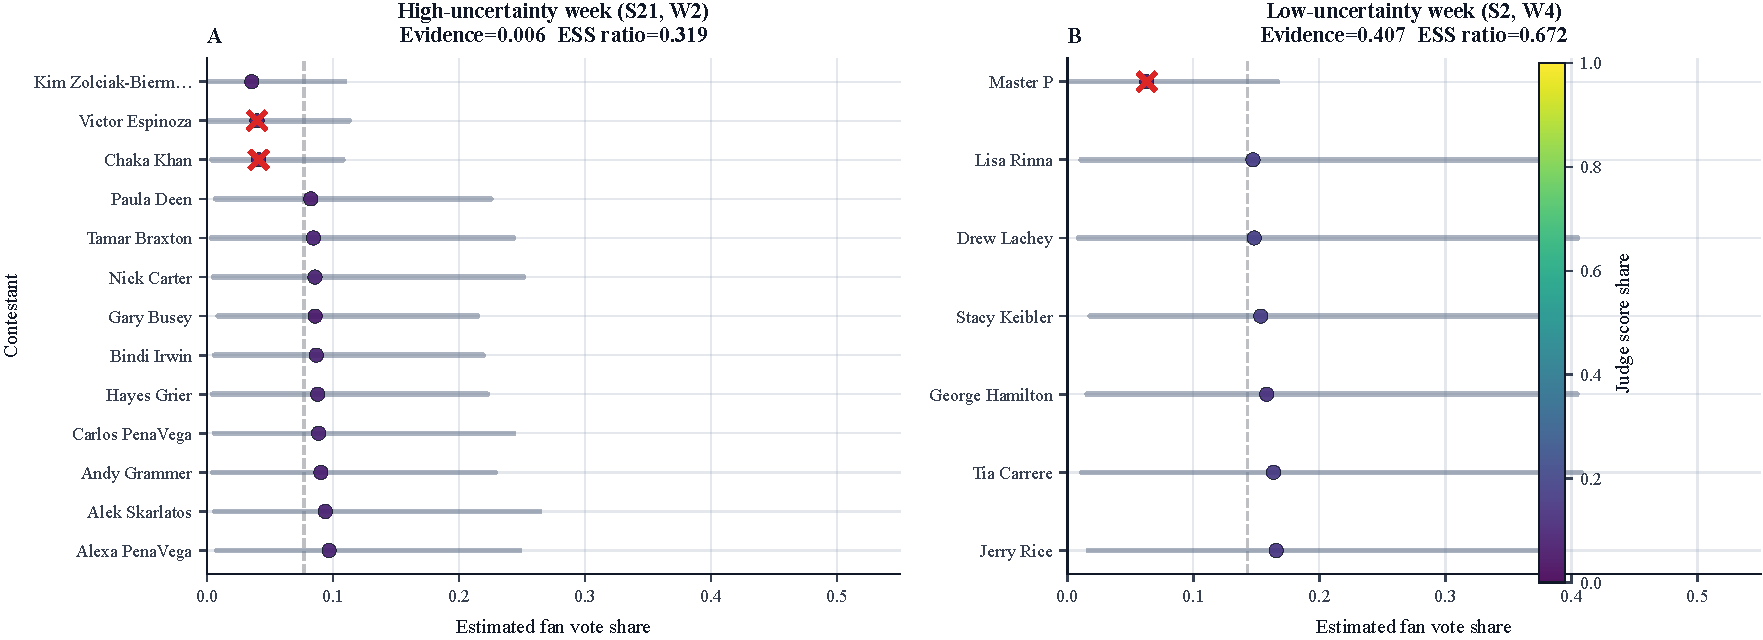
\includegraphics[width=0.96\linewidth]{../outputs/figures/q1/pdf/q1_fan_share_intervals.pdf}
	\caption{Q1核心输出示意：观众份额后验区间（用于支撑后续机制对比与仿真）。} 
	\label{fig:q1_fan_share_intervals}
\end{figure}

\subsection{Model Establishment and Solution of Question Two}
Q2在Q1后验输出的基础上，进一步回答“投票汇总机制改变会如何改变淘汰结果”。我们将观众端信号在Percent与Rank两类机制下进行对照，并用两张图把差异从“定位（哪一周最分歧）”与“分布（差异是系统性还是偶发）”两条视角串联起来。

\paragraph{Counterfactual rule implementation}
在每个\texttt{season$\times$week}上，令当周需要退出的人数为$k$（由\texttt{eliminated\_this\_week}与\texttt{count\_withdraw\_as\_exit}共同确定）。
Percent机制下合成得分与预测退出集合为：
\begin{equation}
S_i = \alpha\,J_i + (1-\alpha)\,\widehat p_i,\qquad \widehat{\mathcal{E}}_{\mathrm{percent}}=\text{argmin}_{|\mathcal{E}|=k} S_i.
\end{equation}
Rank机制下合成排名为：
\begin{equation}
R_i = \alpha\,\mathrm{rank}(J_i) + (1-\alpha)\,\mathrm{rank}(\widehat p_i),\qquad \widehat{\mathcal{E}}_{\mathrm{rank}}=\text{argmax}_{|\mathcal{E}|=k} R_i.
\end{equation}
为避免上游缺失导致静默失败，若Q1在当周某些选手的\texttt{fan\_share\_mean}缺失，实现会回退到均匀分布并在输出中记录缺失统计。

\paragraph{Judge Save variant}
当$k=1$时，我们额外实现Judge Save变体：先按Percent/Rank得到bottom2，再由评委分（\texttt{judge\_score\_total}）决定淘汰其中技术更差者。

\paragraph{Inputs/Outputs (mainline artifacts)}
Q2直接读取\texttt{outputs/predictions/mcm2026c\_q1\_fan\_vote\_posterior\_summary.csv}，并写出\texttt{outputs/tables/mcm2026c\_q2\_mechanism\_comparison.csv}作为赛季层对比汇总（含\texttt{diff\_weeks\_percent\_vs\_rank}与各类匹配率）。周层比较明细在\texttt{outputs/tables/mcm2026c\_q2\_week\_level\_comparison\_percent.csv}与\texttt{outputs/tables/mcm2026c\_q2\_week\_level\_comparison\_rank.csv}中，可用于逐周复核。

\begin{figure}[H]
    \centering
    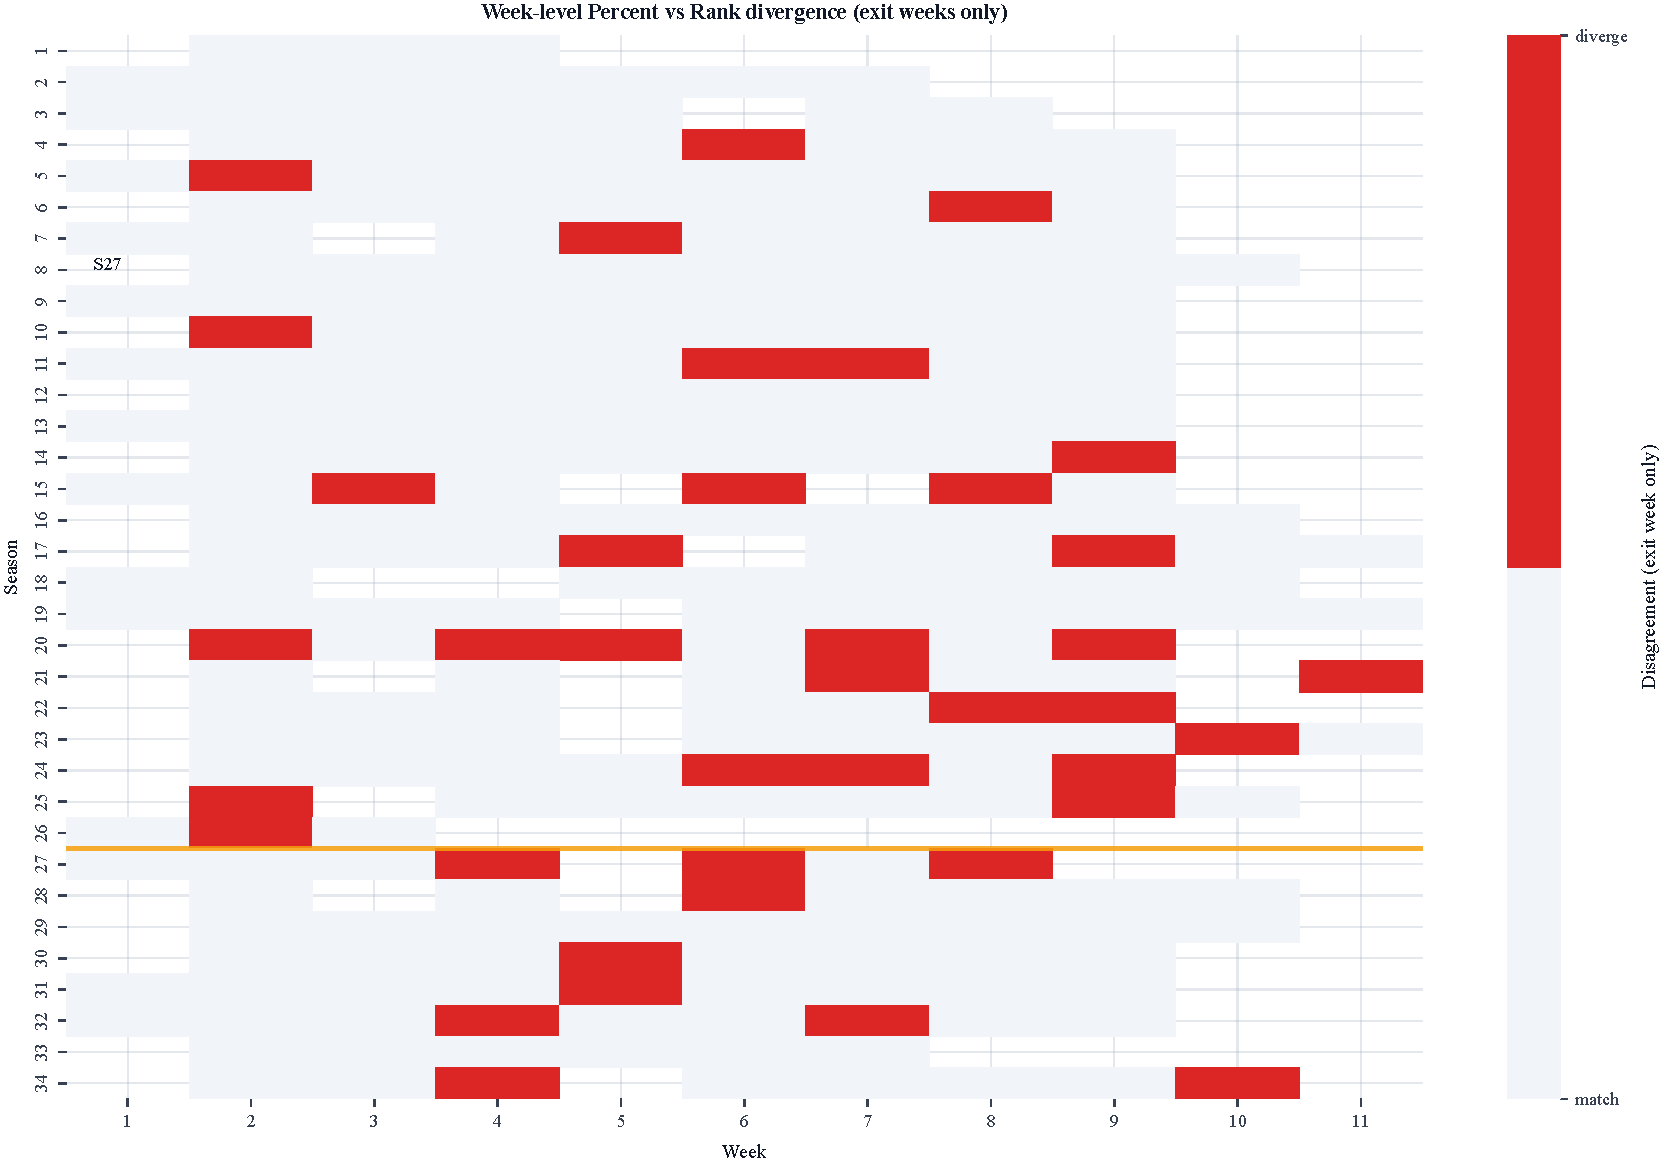
\includegraphics[width=0.96\linewidth]{../outputs/figures/q2/pdf/q2_week_level_divergence_heatmap.pdf}
    \caption{Q2周层分歧定位（Model Building视角）：识别Percent与Rank在何时产生最大分歧，为反事实模拟提供切入点。}
    \label{fig:q2_week_level_divergence_heatmap_mb}
\end{figure}

\begin{figure}[H]
    \centering
    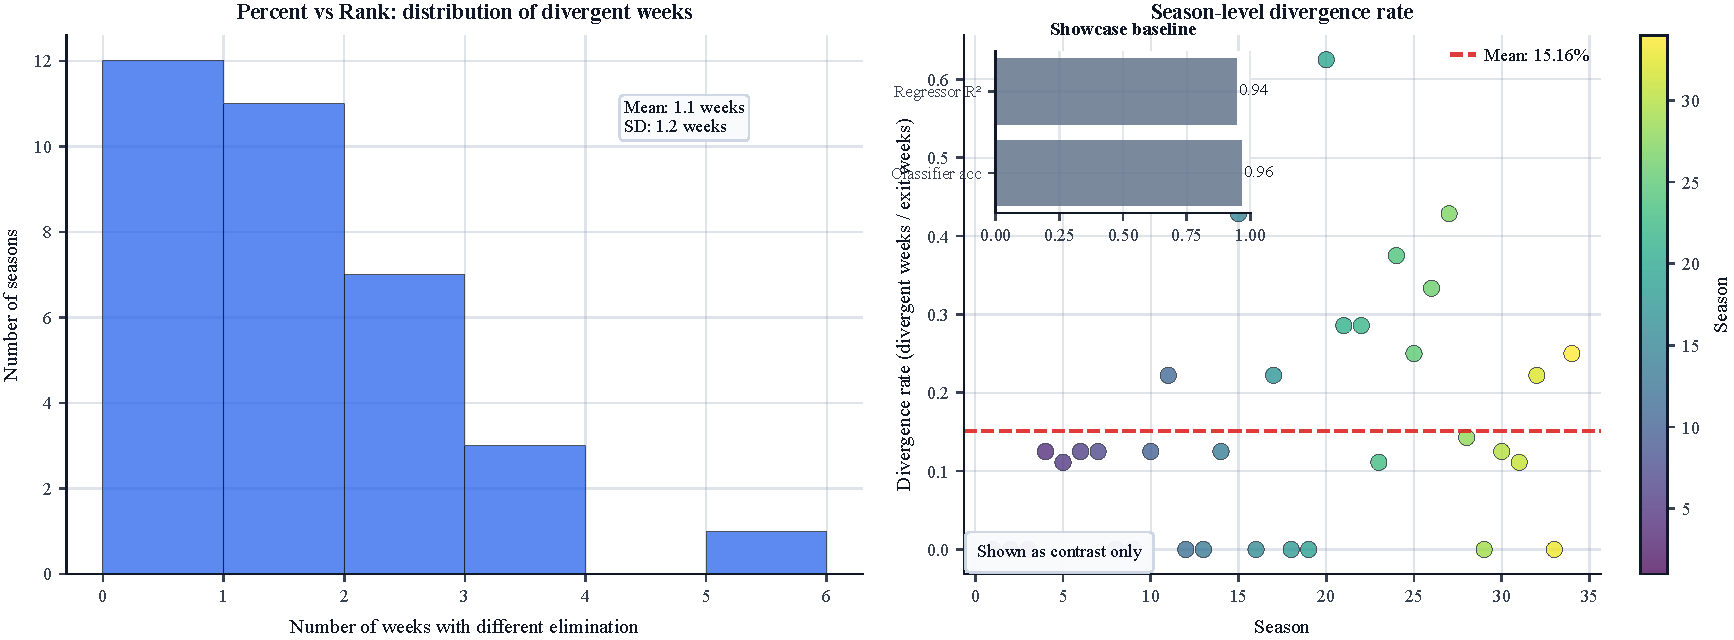
\includegraphics[width=0.92\linewidth]{../outputs/figures/q2/pdf/q2_mechanism_difference_distribution.pdf}
    \caption{Q2机制差异分布（Model Building视角）：检验差异是否集中在少数极端周，避免仅凭个例下结论。}
    \label{fig:q2_mechanism_difference_distribution_mb}
\end{figure}

\subsection{Model Establishment and Solution of Question Three}
Q3旨在回答“哪些因素驱动选手在评委线（technical）与观众线（fan）上的相对优势”。我们在同一数据口径下分别对两条信号建模，并用可解释的系数比较来呈现不同因素的方向与大小。

\paragraph{Two-line modeling strategy}
实现中我们构造赛季级数据集：
(1) 技术线因变量为\texttt{judge\_score\_pct\_mean}（在场周的均值）；
(2) 人气线因变量为\texttt{fan\_vote\_index\_mean}（Q1后验汇总在场周的均值）。
核心协变量包含年龄（含二次项）、行业、是否美国选手、州人口对数等。

\paragraph{Uncertainty propagation}
由于人气线来自Q1推断，必须传播不确定性。实现中由Q1给出的\texttt{fan\_vote\_index\_p05/p95}近似周级标准差，并聚合为赛季均值的不确定度；随后在\texttt{n\_refits}次重拟合中对人气线因变量做扰动抽样，从而给出系数区间与稳定性证据（\texttt{fan\_refit\_coeff\_draws.csv}与\texttt{fan\_refit\_stability.csv}）。

\paragraph{Inputs/Outputs (mainline artifacts)}
Q3读取\texttt{data/processed/dwts\_weekly\_panel.csv}与\texttt{data/processed/dwts\_season\_features.csv}，并将Q1的后验汇总按赛季聚合为观众线因变量；随后拟合混合效应模型（失败时回退OLS）并写出\texttt{outputs/tables/mcm2026c\_q3\_impact\_analysis\_coeffs.csv}。此外，\texttt{outputs/tables/mcm2026c\_q3\_fan\_refit\_coeff\_draws.csv}与\texttt{outputs/tables/mcm2026c\_q3\_fan\_refit\_stability.csv}用于传播Q1不确定性并诊断系数稳定性。

\begin{figure}[H]
    \centering
    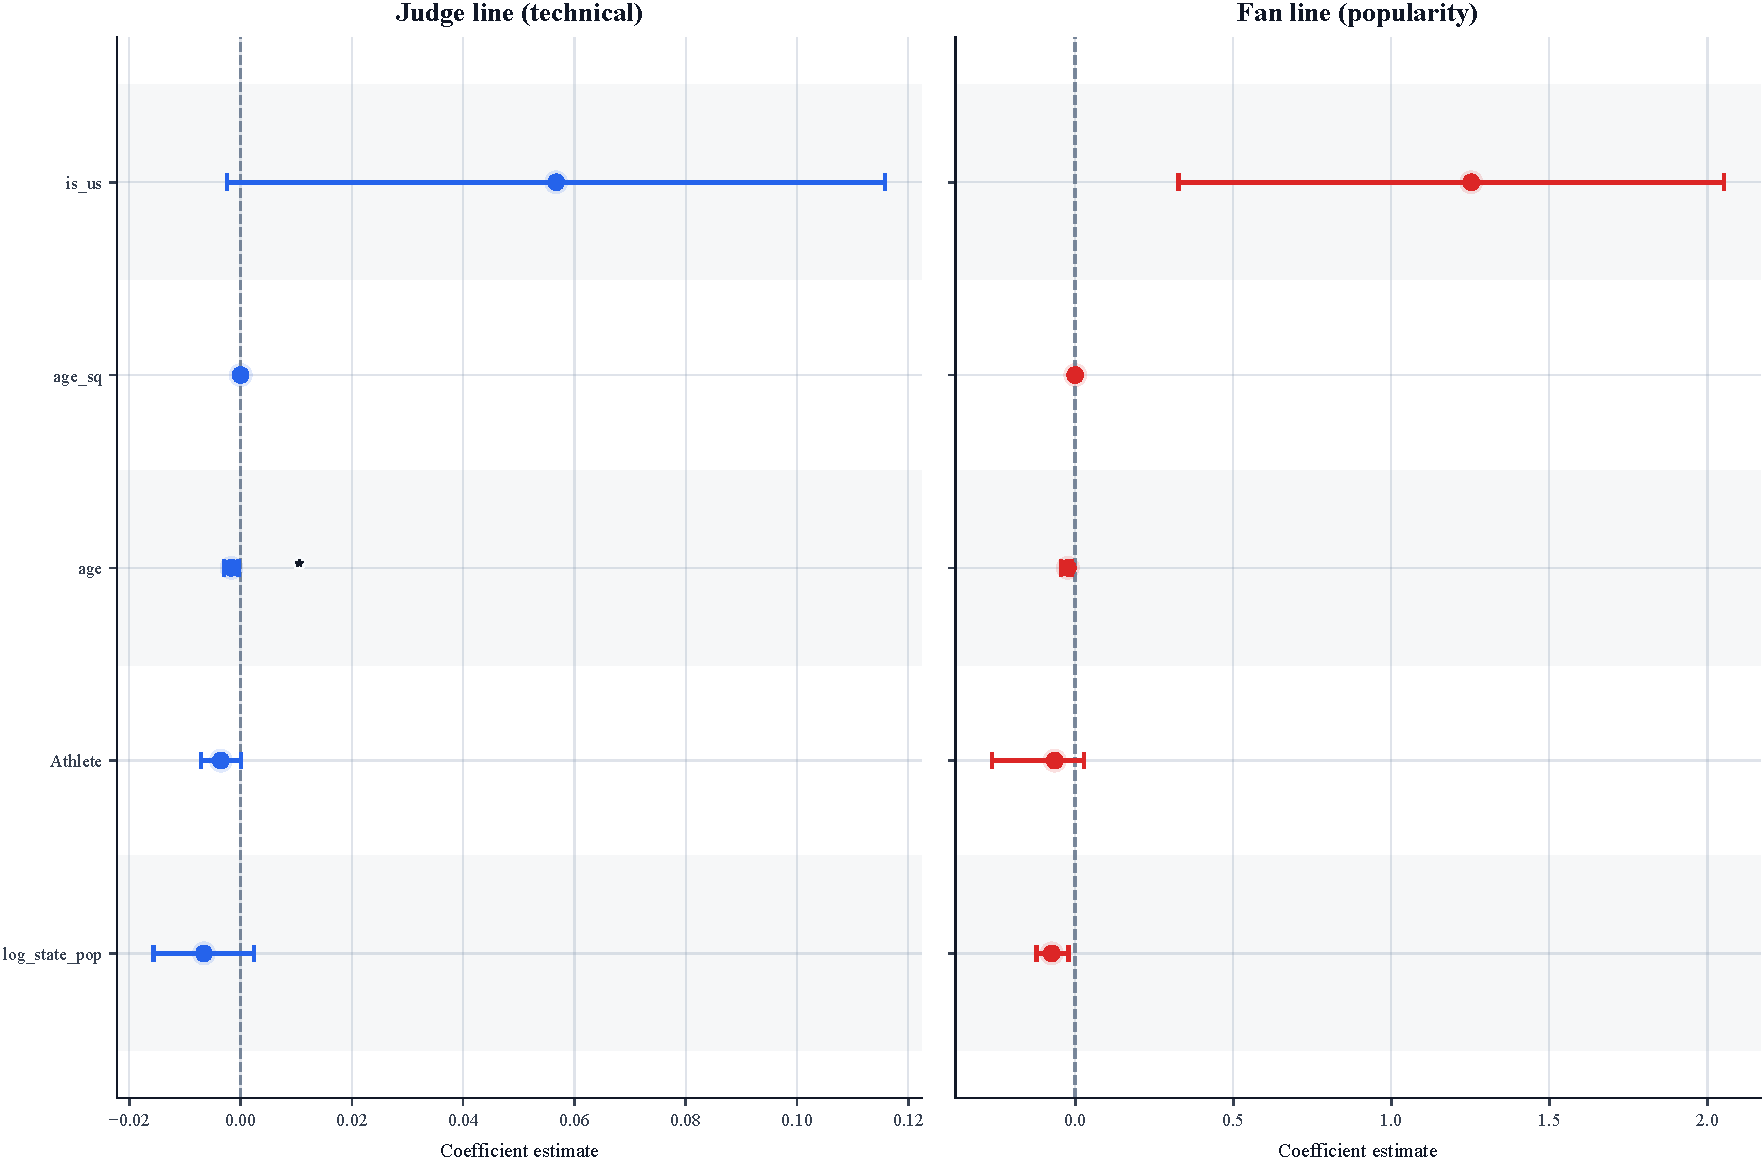
\includegraphics[width=0.98\linewidth]{../outputs/figures/q3/pdf/q3_judge_vs_fan_forest_plot.pdf}
    \caption{Q3关键证据（系数森林图）：对比评委线与观众线的核心协变量效应与区间，突出“同一因素在两条线上的异同”。}
    \label{fig:q3_judge_vs_fan_forest_plot}
\end{figure}

\begin{figure}[H]
    \centering
    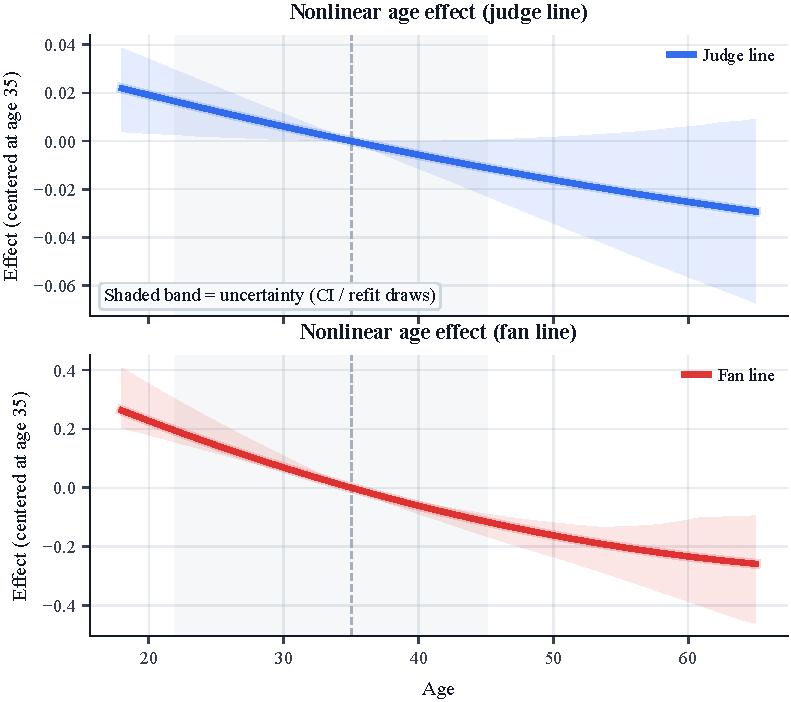
\includegraphics[width=0.92\linewidth]{../outputs/figures/q3/pdf/q3_age_effect_curves.pdf}
    \caption{Q3非线性年龄效应：上为评委线、下为观众线，曲线以35岁为中心化基准，阴影带表示不确定性，并标注拐点位置。}
    \label{fig:q3_age_effect_curves}
\end{figure}

\subsection{Model Establishment and Solution of Question Four}
Q4将Q2的反事实比较进一步扩展到压力测试：我们对不同强度的异常冲击进行模拟，观察各机制的失效概率随压力的变化轨迹，从而把“在正常情况下有效”与“在异常冲击下仍稳健”区分开来。

\paragraph{Simulation loop (season replay)}
实现中对每个赛季做“按周重放”：每周根据题面\texttt{eliminated\_this\_week}/\texttt{withdrew\_this\_week}确定需要退出的人数，并在候选机制下选择退出者更新在场集合；直至决赛周选出冠军。

\paragraph{Fan uncertainty sampling}
在每次模拟中，观众份额不是固定点估计，而是由Q1后验区间构造的log-normal扰动抽样（由\texttt{sigma\_scale}控制强度），以此将Q1不确定性传播到Q4。

\paragraph{Stress tests and robustness attacks}
为评估“极端动员型”冲击，我们对\texttt{outlier\_mult}设定多档压力测试；并可选开启扩展攻击策略（\texttt{robustness\_attacks}），在输出表中形成\texttt{robust\_fail\_rate\_*}列，用于展示不同攻击假设下的失效率区间。

\paragraph{Outputs}
Q4主表\texttt{mcm2026c\_q4\_new\_system\_metrics.csv}同时包含：
(1) 冠军随机性（\texttt{champion\_mode\_prob}与\texttt{champion\_entropy}）；
(2) 技术保护（\texttt{tpi\_season\_avg}及其bootstrap区间）；
(3) 观众表达（\texttt{fan\_vs\_uniform\_contrast}）；
(4) 鲁棒性（\texttt{robust\_fail\_rate}及扩展攻击列），并配套生成Q4图证用于决策表达。

\paragraph{Inputs/Outputs (mainline artifacts)}
Q4读取\texttt{outputs/predictions/mcm2026c\_q1\_fan\_vote\_posterior\_summary.csv}并基于\texttt{src/mcm2026/config/config.yaml}中的\texttt{dwts.q4}参数（\texttt{n\_sims}、\texttt{outlier\_mults}、\texttt{bootstrap\_b}等）进行机制评估。核心指标写入\texttt{outputs/tables/mcm2026c\_q4\_new\_system\_metrics.csv}，并在\texttt{outputs/tables/mcm2026c\_q4\_sensitivity\_summary.csv}中聚合为机制层对比；图\ref{fig:q4_robustness_curves_mb}展示了鲁棒性失败率随压力增强的变化曲线。

\begin{figure}[H]
    \centering
    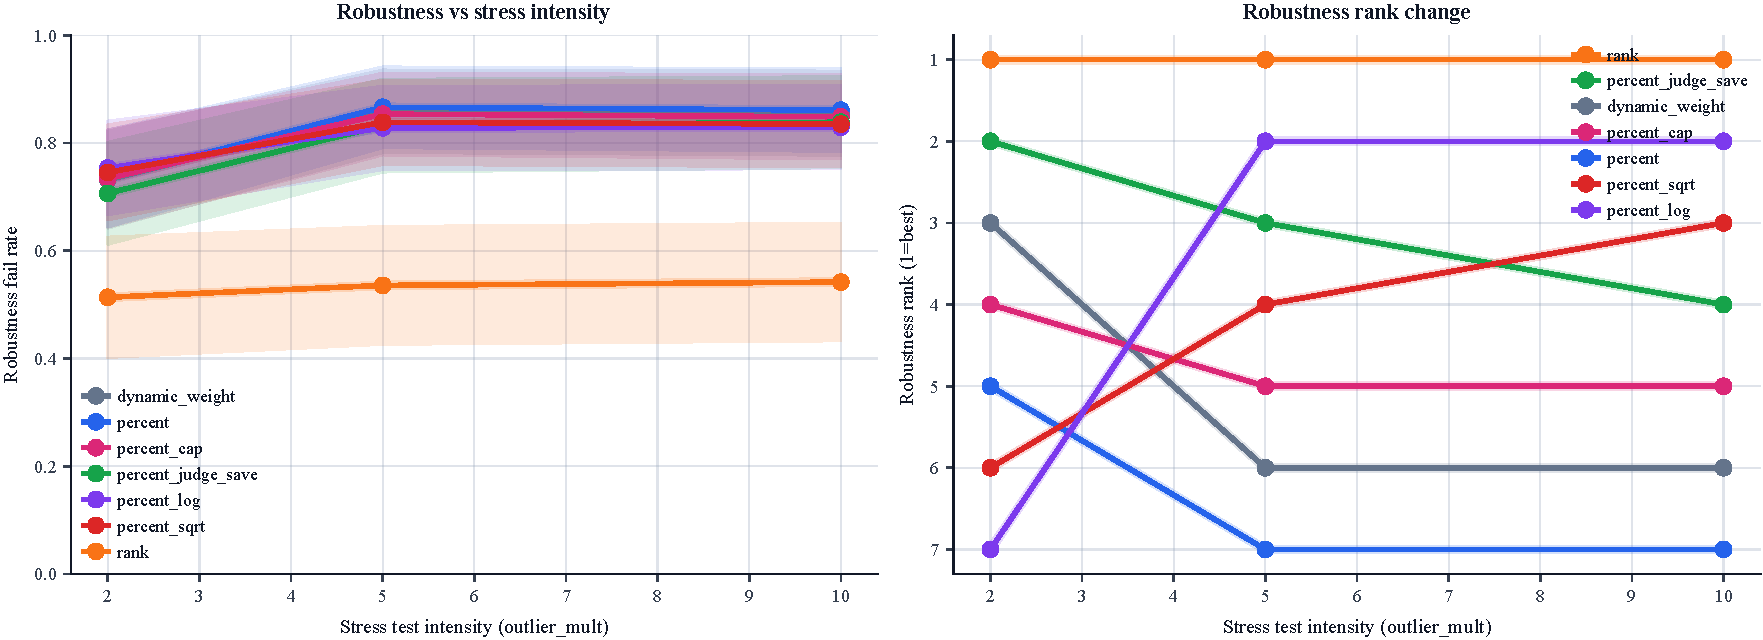
\includegraphics[width=0.96\linewidth]{../outputs/figures/q4/pdf/q4_robustness_curves.pdf}
    \caption{Q4鲁棒性曲线（Model Building视角）：不同机制在压力增强下的失效概率轨迹，用于比较稳健性。}
    \label{fig:q4_robustness_curves_mb}
\end{figure}